\appendix

\section{Limitations}
\label{app:limitations}

\paragraph{Standard-parametric coverage is not full industrial CAD.} BenchCAD parts are generated from expert-authored standard-parametric families, not extracted from real engineering repositories.
We mitigate this by (i) anchoring 49\% of families to published ISO/DIN/EN/ASME/IEC specification tables and (ii) including verified Fusion360 Gallery and DeepCAD subsets for OOD comparison, but our parts do not capture the full diversity of proprietary industrial design (e.g.\ hand-drawn manufacturing tolerances, undocumented design intent, assembly information).

\paragraph{Standard-anchored does not mean standard-compliant.} A family declared as \texttt{standard = "ISO 23509"} samples within ISO parameter ranges and enforces inter-parameter relations from the standard, but does not validate against the full set of manufacturing tolerances or material specifications mandated by that standard.

\paragraph{Industrial Common Sense Gap measurement.} Our non-target preservation metric uses voxel IoU on the spatial complement of the targeted feature; this captures most leakage modes but can miss small parametric shifts whose voxel footprint is subthreshold.
\S\ref{app:edit_protocol} discusses the protocol, including a complementary code-AST diff metric we report alongside.

\section{Extended Related Work: CAD Code-Generation and Editing Benchmarks}
\label{app:related_extended}

\paragraph{Code generation.}
DeepCAD~\citep{Wu2021} introduces a 178K-model corpus of Onshape parts encoded as discrete operation tokens; Text2CAD~\citep{Khan2024} extends DeepCAD with 660K natural-language annotations across four abstraction levels. CAD-Coder~\citep{Guan2025} reformulates the same data as CadQuery Python source and applies SFT$+$GRPO with chain-of-thought and Chamfer reward (mean CD $6.54{\times}10^{-3}$ on Text2CAD). The CAD-Recode~\citep{Rukhovich2025}/cadrille~\citep{Kolodiazhnyi2026}/CADEvolve~\citep{Elistratov2026} lineage shares a Qwen2-VL-2B backbone: CAD-Recode fine-tunes on 1M sketch-and-extrude scripts (DeepCAD IoU 92.0); cadrille adds multi-modal inputs and Dr.CPPO online RL with piecewise IoU reward (DeepCAD IoU 92.2, Fusion360 IoU 84.6, 0.0\% invalidity); CADEvolve expands the corpus to $\sim$1.3M scripts via an LLM-driven evolutionary loop covering extrude/revolve/loft/sweep/fillet/chamfer/shell/Boolean/patterns (DeepCAD IoU 92.6) --- broadening the operation distribution but still without helical sweeps or parametric involute-gear construction. The CADEvolve Hugging Face release contains only sentence embeddings (\texttt{.npy}), not the source code, so its full operation surface is not directly auditable; the public GitHub repo ships only $46$ hand-written seed programs.

\paragraph{Editing.}
CADPrompt~\citep{Alrashedy2025} introduces 200 NL$\to$CadQuery prompts scored via point-cloud distance and bounding-box IoU after ICP alignment --- two orders of magnitude smaller than BenchCAD-Edit (17{,}900), without family taxonomy or difficulty stratification, and with potential scale leakage from absolute mm cues and axis-aligned IoU. CAD-Editor~\citep{CADEditor2025} trains a locate-then-infill editor entirely on synthetic edits, but releases no held-out human-verified edit benchmark. CADialogue~\citep{CADialogue2025} evaluates ten edit tasks in a conversational CAD interface, but does not release the eval set. HistCAD~\citep{Dong2026} evaluates constraint preservation under FreeCAD edits, but at the sketch-constraint rather than executable-program level. BenchCAD-Edit is, to our knowledge, the first public CAD editing benchmark with execution-verified before/after CadQuery pairs, preservation-aware metrics, and balanced cross-family edit-category coverage.

\section{Full Comparison Against Prior CAD Code-Generation Work}
\label{app:cmp_prior}

Table~\ref{tab:cmp_prior} provides the full per-axis comparison referenced in \S\ref{sec:related}, including all evaluation-side properties (\#Industrial families, \#Std codes, \#Distinct CQ ops, Adv ops, Edit / QA tasks, \#Eval models) across DeepCAD, Fusion360 Gallery, Text2CAD, CADPrompt, CAD-Coder, CAD-Recode, cadrille, and CADEvolve.

\begin{table*}[t]
\centering
\small
\setlength{\tabcolsep}{5pt}
\caption{\textbf{BenchCAD versus prior CAD code-generation work.} BenchCAD is a \emph{unified, capability-decomposed evaluation framework} for large-model CAD reasoning, distinct in purpose from the CadQuery-VLM lineage (CAD-Recode, cadrille, CADEvolve) which releases training corpora alongside small fine-tuned models (Qwen 1.5B--2B) saturating $\sim$92\% IoU on legacy sketch+extrude splits. \textbf{Type:} \emph{C+M} = corpus+model, \emph{D} = dataset, \emph{B} = benchmark. \textbf{\#Fam.} = named industrial part families with explicit functional identity. \textbf{\#Std} = distinct ISO/DIN/EN/ASME/IEC specification codes. \textbf{\#Ops} = distinct CadQuery API methods exercised in the released corpus (static analysis of every released \texttt{.py}; see Appendix~\ref{app:ops}). \textbf{Adv} = all four advanced operation families (helix, loft/sweep, twist-extrude, parametric involute-gear) exercised. $\checkmark$ = supported, p.\ = partial, -- = absent.}
\label{tab:cmp_prior}
\begin{tabular}{lccrrrrccc}
\toprule
Benchmark & Yr & Type & \#Sam. & \#Fam. & \#Std & \#Ops & Adv & Edit & QA \\
\midrule
DeepCAD~\citep{Wu2021}                   & '21 & C+M & 178K  & -- & 0  & 4   & --   & --   & --   \\
Fusion360 G.~\citep{Willis2021fusion}    & '21 & D   & 8K    & -- & 0  & 6   & --   & --   & --   \\
Text2CAD~\citep{Khan2024}                & '24 & C+M & 170K  & -- & 0  & 17  & --   & --   & --   \\
CADPrompt~\citep{Alrashedy2025}          & '25 & B   & 200   & -- & 0  & --  & p.\  & --   & --   \\
CAD-Coder~\citep{Guan2025}               & '25 & C+M & 110K  & -- & 0  & 4   & --   & p.\  & --   \\
CAD-Recode~\citep{Rukhovich2025}         & '25 & C+M & 1M+7K & -- & 0  & 18  & --   & p.\  & seq.\\
cadrille~\citep{Kolodiazhnyi2026}        & '26 & C+M & 1M+7K & -- & 0  & 18  & --   & --   & --   \\
CADEvolve~\citep{Elistratov2026}         & '26 & C+M & 2.7M  & -- & 0  & 25  & p.\  & --   & --   \\
\midrule
\textbf{BenchCAD (ours)} & \textbf{'26} & \textbf{D+B} & \textbf{17{,}900} & \textbf{106} & \textbf{43} & \textbf{49} & $\checkmark$ & $\checkmark$ & $\checkmark$ \\
\bottomrule
\end{tabular}
\end{table*}

\section{Standard Codes Covered}
\label{app:standards}
Table~\ref{tab:standards} reports the standards grounding of BenchCAD. 
Nearly half of all families, 52/106 (49\%), are tied to ISO, DIN, EN, ASME, or IEC specification tables, so their dimensions are sampled from real engineering ranges rather than arbitrary shapes. 
The remaining 54 custom families cover bespoke industrial parts without a formal standard, while still using analogous proportional design rules.

\begin{table}[t]
\centering
\small
\caption{\textbf{Standard-anchored families.} 55\% of BenchCAD families bind their parameters to ISO/DIN/EN/ASME/IEC specification tables, sampling at values drawn from real engineering ranges rather than arbitrary geometry. The bottom row lists the 47 custom families covering bespoke industrial parts (twisted brackets, lobed knobs) governed by analogous proportional rules without formal standards.}
\label{tab:standards}
\begin{tabular}{llr}
\toprule
Standard & Codes covered (sample) & \#Fam. \\
\midrule
ISO   & 22, 113, 272, 1234, 2339, 2936, 10828, 23509, \ldots & 22 \\
DIN   & 338, 471/472, 580, 5480, 2095, 8187, 71412, \ldots    & 28 \\
EN    & 10034, 10056, 10219, 10279                            & 4  \\
ASME  & B1.20.1, B16.5, B16.9                                 & 3  \\
IEC   & 60072-1, 60086                                        & 2  \\
\midrule
\textbf{Total standard-anchored}   &                              & \textbf{59 (55\%)} \\
Custom (no formal standard)        &                              & 47 \\
\bottomrule
\end{tabular}
\end{table}


\section{Dataset Generation Details}
\label{app:datagen}

\paragraph{Subfamilies.} A family may further branch into one or more \emph{subfamilies} that capture mating, assembly, or construction variants of the same part type --- for instance, a threaded-fastener family may split into male (\texttt{bolt}) and female (\texttt{nut}) subfamilies that share the same thread/pitch parameter table but differ in build chain; a retaining-ring family may split into internal (groove inside a bore) and external (groove on a shaft) variants; a thread family may split into single- and multi-start helices. Subfamilies reuse their parent family's parameter schema and standard-table anchoring, but specify their own deterministic builder. They are sampled and rendered independently, so a single named family in the per-family analysis can contribute several subfamily$\times$tier buckets to the verified release.

\paragraph{Difficulty tiers.} Each (sub)family exposes three tiers --- \emph{easy} / \emph{medium} / \emph{hard} --- defined by parameter complexity. Easy uses default parameter ranges with optional features disabled (e.g., a coil spring with constant pitch and no end treatment). Medium expands parameter ranges and enables a subset of optional features. Hard activates all optional features and uses extreme but still standard-compliant parameter ranges (e.g., variable pitch with closed-and-ground spring ends), exercising the more advanced construction operations of the family. Sampling is balanced approximately uniformly across tiers within each (sub)family.

\paragraph{Sandbox failure-mode taxonomy.} Each generated CadQuery program is executed in a sandbox subprocess; records hitting any of the following are quarantined and excluded from the release: (i) \emph{parse / import error} --- the program fails Python parsing or CadQuery API resolution; (ii) \emph{runtime exception} --- a CadQuery call raises (e.g., on a non-positive radius or an empty selector); (iii) \emph{timeout} --- execution exceeds a 30\,s wall-clock budget, typically caused by pathological boolean or sweep construction; (iv) \emph{degenerate volume} --- the resulting solid has $\leq 10^{-6}$\,mm$^3$ volume or an inverted (negative-determinant) transformation chain. Programs surviving all four checks are rendered into multi-view images and routed past a domain expert for visual sign-off; only records passing every stage enter the release.

\section{Full Per-Model Per-Task Results}
\label{app:full_results}

Table~\ref{tab:dataset} reports the dataset composition; Table~\ref{tab:capability} maps each task to its sub-capability subset; Tables~\ref{tab:main_eval_qa_img} and~\ref{tab:main_eval_qa_code} report the per-model QA leaderboard (Vision QA / Code QA); Table~\ref{tab:family_cliff} stratifies \texttt{img2cq} by family difficulty. The unified Vision2Code leaderboard (Table~\ref{tab:codegen_unified}) is in the main body.

\begin{table}[t]
\centering
\small
\caption{\textbf{BenchCAD dataset composition.} Three released datasets: the verified CadQuery code core (17{,}900 parts spanning 106 families, each with parametric source, executable STEP, four canonical-view renders, parameter JSON, and op list), the paired QA bank (2{,}400 questions evaluated under both visual and code conditioning), and the Edit subset (748 before/after pairs).}
\label{tab:dataset}
\begin{tabular}{lrrl}
\toprule
Dataset & \#Records & \#Families & GT artefacts \\
\midrule
BenchCAD                     & 17{,}900             & 106 & code $\cdot$ STEP $\cdot$ 4 views $\cdot$ params $\cdot$ ops \\
BenchCAD-QA (paired img/code)& 2{,}400 $\times 2$   & 106 & question $+$ gold answer \\
BenchCAD-Edit                & 748                  & 106 & before/after $+$ NL instruction \\
\bottomrule
\end{tabular}
\end{table}


\begin{table}[t]
\centering
\small
\caption{\textbf{Capability decomposition.} BenchCAD's five tasks isolate the three sub-capabilities along the image$\to$code causal chain: $C_1$ visual + 3D reconstruction, $C_2$ geometric$\to$parametric abstraction, and $C_3$ parametric$\to$code synthesis. Score differences across paired tasks (e.g.\ \texttt{qa\_img}$-$\texttt{qa\_code}) directly diagnose which capability is the bottleneck. ``part.'' indicates partial coverage (the original code constrains, but does not eliminate, the corresponding sub-capability).}
\label{tab:capability}
\begin{tabular}{llccc}
\toprule
Task & Input $\to$ Output & $C_1$ vision & $C_2$ param. & $C_3$ code \\
\midrule
\texttt{img2cq}    & 4 views $\to$ code              & \cmark & \cmark & \cmark \\
\texttt{qa\_img}   & 4 views $+$ Q $\to$ number      & \cmark & \cmark & --     \\
\texttt{qa\_code}  & code $+$ Q $\to$ number         & --     & \cmark & --     \\
\texttt{edit\_img} & views $+$ code $+$ instr $\to$ code  & \cmark & part.  & \cmark \\
\texttt{edit\_code}& code $+$ instr $\to$ code       & --     & part.  & \cmark \\
\bottomrule
\end{tabular}
\end{table}


\begin{table*}[t]
\centering
\small
\setlength{\tabcolsep}{5pt}
\renewcommand{\arraystretch}{1.15}
\caption{\textbf{Main evaluation on BenchCAD-QA (\texttt{qa\_code} modality), by capability axis.} Per-model accuracy on the code-conditioned QA bank across the same four capability axes as Table~\ref{tab:main_eval_qa_img}. The two tables share questions and capability-axis definitions; only the conditioning modality differs (rendered images vs.\ source CadQuery). Score differences across the matched pair isolate the cost of replacing direct code access with visual recognition --- the \textbf{Holistic Spatial and Detailing Deficit}.}
\label{tab:main_eval_qa_code}
\begin{tabular}{l c c c c c}
\toprule
Model
 & \shortstack{Cadquery Code\\Recognition $\uparrow$ }
 & \shortstack{CAD Operation\\Understanding $\uparrow$ }
 & \shortstack{Industrial Parametric\\Abstraction $\uparrow$ }
 & \shortstack{Spatial\\Reasoning $\uparrow$ }
 & \shortstack{Total\\score $\uparrow$ } \\
\midrule
opus-4.7         & 0.868 & 0.800 & 0.793 & 0.595 & 0.801 \\
opus-4.7-thinking            & 0.891 & 0.781 & 0.851 & 0.632 & 0.829 \\
gemini-3.1-pro  & \textbf{0.914} & 0.782 & 0.867 & 0.537 & 0.836 \\
gemini-3.1-pro-thinking     & 0.907 & 0.783 & \textbf{0.876} & 0.537 & \textbf{0.838} \\
gpt-4o                              & 0.865 & 0.593 & 0.732 & 0.688 & 0.726 \\
gpt-5.3-chat-latest                 & 0.879 & \textbf{0.805} & 0.815 & 0.731 & 0.823 \\
gpt-5.3-thinking                    & 0.885 & 0.802 & 0.811 & 0.730 & 0.821 \\
moonshot-v1-128k-v     & 0.842    & 0.551    & 0.692    & \textbf{0.792}    & 0.700 \\                                                                       
  moonshot-v1-8k-v       & 0.772    & 0.603    & 0.555    & 0.536    & 0.620 \\               
openai-o3                & 0.804    & 0.701    & 0.689    & 0.492    & 0.708 \\                                                                
  google-gemma-4-31b-it    & 0.791    & 0.674    & 0.606    & 0.528    & 0.664 \\                                                                
  openai-gpt-oss-120b      & 0.790    & 0.732    & 0.656    & 0.379    & 0.689 \\
  nvidia-nemotron-3-120b   & 0.771    & 0.660    & 0.661    & 0.293    & 0.671 \\       
\midrule
\textit{blank code (baseline)}     & 0.040    & 0.257    & 0.290    & 0.420    & 0.223    \\
\bottomrule
\end{tabular}
\end{table*}


\begin{table}[t]
\centering
\small
\setlength{\tabcolsep}{6pt}
\renewcommand{\arraystretch}{1.05}
\caption{\textbf{Vision2Code unified leaderboard.} Specialist CAD lineage (cadrille / CADEvolve), frontier MLLMs, and our open Qwen3-VL-2B trained baseline. All BenchCAD scores on BenchCAD-Lite. \emph{(\,$\dagger$\,)} Ours-SFT-IID is evaluated on the IID split (all 106 families seen at train time); all other rows are OOD on BenchCAD by construction (specialist lineage and frontier MLLMs never saw BenchCAD; ours-SFT-OOD / +RL hold out 10 mech.-transmission families). Essential-op recall is the fraction of ground-truth essential operations (helix / sweep / loft / twist-extrude / parametric involute-gear) recovered by the prediction.}
\label{tab:codegen_unified}
\begin{tabular}{@{}lcccl@{}}
\toprule
Model                                                  & DeepCAD IoU      & BenchCAD IoU            & Ess.\ op recall  & Notes \\
\midrule
\multicolumn{5}{l}{\emph{Specialist CAD lineage ($\sim$2B, OOD on BenchCAD)}} \\
cadrille-RL~\citep{Kolodiazhnyi2026}                   & 0.919            & 0.273                   & --               & sketch+ext, 1M \\
CADEvolve~\citep{Elistratov2026}                       & 0.923            & 0.039                   & --               & extended, 2.7M \\
\midrule
\multicolumn{5}{l}{\emph{Frontier MLLMs (BenchCAD-Lite, by def.\ OOD)}} \\
gpt-4o                                                 & --               & 0.188                   & 0.468            & \\
gpt-5.3 (thinking)                                     & --               & 0.207                   & 0.455            & \\
claude-opus-4.7 (thinking)                             & --               & 0.267                   & 0.471            & \\
gemini-3.1-pro (thinking)                              & --               & \textbf{0.279}          & \textbf{0.567}   & strongest frontier \\
\midrule
\multicolumn{5}{l}{\emph{Ours --- Qwen3-VL-2B, 9 GPU-h on $8{\times}$A800-80GB}} \\
SFT (IID, 106 fam.\ seen)$^{\dagger}$                  & --               & \textbf{0.650}          & \textbf{0.950}   & dataset learnable on 2B \\
SFT (OOD, 10 fam.\ held out)                           & --               & 0.180                   & 0.200            & generalisation gap \\
\quad $+$ RL ($r{=}0.2\,\mathrm{ess}{+}0.8\,\mathrm{IoU}$) & --             & 0.350                   & 0.450            & RL partial recovery \\
\bottomrule
\end{tabular}
\end{table}


\begin{table}[t]
\centering
\small
\caption{\textbf{The Family Cliff.} \texttt{img2cq} pass rate (\%) split by family difficulty tier. Even the strongest reasoning model collapses on the hard tier, exhibiting a $>$45-point gap from easy. The 26 hard-tier families exercise advanced operations (helical sweeps, twist-extrusion, lofted Booleans) and parametric constraints (gear module--tooth--pitch consistency, spring free-length--turn-count coupling) that no evaluated model reliably preserves. \textcolor{red}{Numbers are placeholders.}}
\label{tab:family_cliff}
\begin{tabular}{lrrrr}
\toprule
Model & Easy (40 fam.) & Medium (40 fam.) & Hard (26 fam.) & $\Delta$ E$-$H \\
\midrule
GPT-5.3 (think)          & 68 & 42 & \textbf{20} & \textbf{48} \\
Claude Opus 4.7 (think)& 65 & 40 & 19 & 46 \\
GPT-4o                 & 52 & 28 & 9  & 43 \\
Qwen2.5-VL-72B         & 38 & 18 & 5  & 33 \\
InternVL3-1B           & 15 & 4  & 1  & 14 \\
\bottomrule
\end{tabular}
\end{table}


\section{CAD Operational Blindspot: Per-Operation Recall}
\label{app:op_gap_full}
Table~\ref{tab:op_recall} reports the recall of operations.

\begin{table}[t]
    \centering
    \small
    \setlength{\tabcolsep}{4pt}
    \caption{\textbf{TODO Per-operation recall on Vision2Code} with paired comparison of gpt-5.3 (chat-latest) vs gpt-5.3-thinking.              
    Thinking-mode degrades both macro recall (advanced: 25.2 → 22.8, all: 35.1 → 32.3) and execution rate (69.5 → 
    67.5), against the common expectation that inference-time reasoning monotonically helps. Looking inside the per-op 
    deltas reveals a structural trade: thinking improves recall on composition-choice and finishing operations that 
    benefit from explicit planning (loft +17.6, polygon +18.2, fillet +12.0, rarray +7.2) but degrades on direct       
    boolean and scaffolding operations (cut −11.9, cutBlind −10.5, workplane −8.9, sweep −7.7, box −7.7, union −5.6). 
    The net effect is a synthesis-execution trade-off
    — the model thinks more about which high-level op
    to call, while writing the surrounding boilerplate
    less reliably.}
    \label{tab:op_recall}
  \begin{tabular}{lrrr}                                             
  \toprule                                                                                 
  Operation & gpt-5.3 & gpt-5.3-thk & $|\text{GT}|$ \\                                                             
  \midrule                                                                                                             
  \multicolumn{4}{l}{\emph{Basic ops (shared with prior corpora: cad-recode / text2cad)}} \\                           
  \texttt{extrude}              & 83.3          & \textbf{84.4} & 90  \\                                               
  \texttt{cut}                  & \textbf{44.1} & 32.2          & 59  \\                                               
  \texttt{union}                & \textbf{65.3} & 59.7          & 72  \\                                               
  \texttt{circle}               & \textbf{78.7} & 77.3          & 75  \\                                               
  \texttt{cylinder}             & 4.5           & \textbf{7.6}  & 66  \\                                               
  \texttt{box}                  & \textbf{42.3} & 34.6          & 78  \\                                               
  \texttt{rect}                 & 63.0          & \textbf{65.2} & 46  \\                                               
  \texttt{workplane}            & \textbf{86.3} & 77.4          & 124 \\                                               
  \midrule                                                                                                             
  \multicolumn{4}{l}{\emph{Advanced ops (BenchCAD-distinguishing)}} \\                                                 
  \texttt{hole}                 & \textbf{60.2} & 55.4          & 83  \\                                               
  \texttt{chamfer}              & \textbf{8.6}  & 4.3           & 70  \\                                               
  \texttt{cutThruAll}           & \textbf{16.2} & 10.8          & 37  \\                                               
  \texttt{revolve}              & \textbf{14.3} & 10.7          & 28  \\                                               
  \texttt{fillet}               & 0.0           & \textbf{12.0} & 25  \\
  \texttt{cutBlind}             & \textbf{36.8} & 26.3          & 19  \\                                               
  \textbf{\texttt{loft}}        & 5.9           & \textbf{23.5} & 17  \\
  \texttt{threePointArc}        & \textbf{6.2}  & 0.0           & 16  \\                                               
  \texttt{rarray}               & 7.1           & \textbf{14.3} & 14  \\                                               
  \textbf{\texttt{sweep}}       & \textbf{53.8} & 46.2          & 13  \\                                               
  \texttt{polygon}              & 54.5          & \textbf{72.7} & 11  \\                                               
  \texttt{makeHelix}            & 12.5          & 12.5          & 8   \\                                               
  \texttt{slot2D}               & 25.0          & 25.0          & 8   \\                                               
  \texttt{polarArray}           & 20.0          & 20.0          & 5   \\                                               
  \texttt{shell}                & \textbf{25.0} & 0.0           & 4   \\
  \texttt{mirrorY}              & 0.0           & 0.0           & 4   \\                                               
  \texttt{sphere}               & 100.0         & 100.0         & 4   \\
  \texttt{cboreHole}            & 0.0           & 0.0           & 3   \\                                               
  \texttt{radiusArc}            & \textbf{33.3} & 0.0           & 3   \\
  \midrule                                                                                                             
  \textbf{Macro recall} (advanced, 19 ops) & \textbf{25.2\%} & 22.8\% & --- \\
  \textbf{Macro recall} (all, 27 ops)      & \textbf{35.1\%} & 32.3\% & --- \\                                         
  \textbf{Exec rate}                       & \textbf{69.5\%} & 67.5\% & --- \\                                         
  \bottomrule                                                                                                          
  \end{tabular}                                                                                                       
                                     
    % \begin{tabular}{lrrrr}
    % \toprule
    % Operation & baseline & ood & iid & $|\text{GT}|/100$ \\
    % \midrule
    % \multicolumn{5}{l}{\emph{Basic ops (shared with prior corpora: cad-recode / text2cad)}} \\
    % \texttt{extrude}              & 100.0 & 91.7  & 95.8  & 24 \\
    % \texttt{cut}                  & 87.2  & 70.2  & 89.4  & 47 \\
    % \texttt{union}                & 91.7  & 41.7  & 79.2  & 24 \\
    % \texttt{circle}               & 82.8  & 79.3  & 96.6  & 29 \\
    % \texttt{cylinder}             & 5.9   & 88.2  & 94.1  & 17 \\
    % \texttt{box}                  & 2.6   & 84.6  & 92.3  & 39 \\
    % \texttt{rect}                 & 5.0   & 65.0  & 90.0  & 20 \\
    % \texttt{workplane}            & 0.0   & 77.4  & 88.7  & 53 \\
    % \midrule
    % \multicolumn{5}{l}{\emph{Advanced ops (BenchCAD-distinguishing)}} \\
    % \textbf{\texttt{revolve}}     & \textbf{0.0} & \textbf{54.8} & \textbf{93.5} & 31 \\
    % \textbf{\texttt{loft}}        & \textbf{0.0} & \textbf{22.2} & \textbf{77.8} &  9 \\
    % \textbf{\texttt{sweep}}       & \textbf{0.0} & \textbf{25.0} & \textbf{75.0} &  8 \\
    % \textbf{\texttt{sweep+helix}} & \textbf{0.0} & \textbf{100.0}& \textbf{50.0} &  2 \\
    % \textbf{\texttt{twistExtrude}}& \textbf{0.0} & \textbf{100.0}& \textbf{100.0}&  1 \\
    % \texttt{fillet}               & 0.0   & 25.0  & 87.5  &  8 \\
    % \texttt{chamfer}              & 0.0   & 85.3  & 85.3  & 34 \\
    % \texttt{shell}                & 0.0   & 80.0  & 100.0 &  5 \\
    % \texttt{hole}                 & 0.0   & 82.8  & 93.1  & 29 \\
    % \texttt{rarray}               & 0.0   & 77.8  & 100.0 &  9 \\
    % \texttt{polarArray}           & 0.0   & 33.3  & 83.3  &  6 \\
    % \midrule
    % \textbf{Macro recall} (16 ops) & \textbf{17.5\%} & \textbf{59.9\%} & \textbf{84.0\%} & --- \\
    % \textbf{Exec rate}             & 90.0\% & 94.0\% & 99.0\%        & --- \\
    % \bottomrule
    % \end{tabular}
    \end{table}

    

\section{Model Training}
\paragraph{SFT training mixture.}
(1) \textbf{iid}: BenchCAD (all 106 families) + extrusion-heavy data (text2cad, cad-recode);
(2) \textbf{ood}: same recipe, 10 mechanical families held out;
(3) \textbf{baseline}: text2cad + cad-recode only (no BenchCAD).
Mixing 33\% BenchCAD / 67\% HQ for (1)/(2); 100\% HQ for (3). Backbone Qwen3-VL-2B.

\paragraph{OOD holdout selection.}
We hold out 10 CAD families sampled uniformly at random from BenchCAD families that are sufficiently represented and the operations are covered in the iid but not in the baseline.

\paragraph{SFT training setup.}
We fine-tune Qwen3-VL-2B-Instruct under a standard supervised code-generation setup. Inputs consist of one rendered view and a textual instruction, and targets are CadQuery programs.We use AdamW with
learning rate $2{\times}10^{-4}$, cosine decay, $2$k warmup steps, weight decay $0.01$ with bf16 precision.

\paragraph{RL training setup.}
We initialize RL from the matching SFT checkpoint: IID-SFT uses the full BenchCAD training set, whereas OOD-SFT excludes the held-out OOD families. RL is trained with a top-$N$ GRPO-style objective without advantage normalization on a mixed prompt pool from BenchCAD, DeepCAD, and Fusion360; in the OOD setting, the held-out families remain excluded. Rewards combine geometric fidelity with an essential-operation term when available. We use learning rate $2{\times}10^{-5}$, 16 rollouts per prompt, and batch size 128.

\begin{table}[t]
\centering
\small
\setlength{\tabcolsep}{5pt}
\renewcommand{\arraystretch}{1.08}
\caption{\textbf{IID--OOD generalization under SFT and RL.}
We report geometric fidelity, execution rate, essential-operation score, and the final score.}
\label{tab:iid_ood}
\begin{tabular}{@{}llccccc@{}}
\toprule
Checkpoint & Split & IoU$\uparrow$ & Exec.$\uparrow$ & Ess.$\uparrow$ & Score$\uparrow$ \\
\midrule
\multirow{2}{*}{ood-sft (A)}
& IID  & 0.577 & 94.6\% & 0.789 & 0.6064 \\
& OOD  & 0.397 & 89.8\% & 0.305 & 0.3776 \\
\midrule
\multirow{2}{*}{ood-rl (B)}
& IID & 0.757 & 99.1\%  & 0.865 & 0.7467 \\
& OOD  & 0.464 & \textbf{100.0\%} & 0.339 & 0.4604 \\
\midrule
\multirow{2}{*}{iid-sft (C)}
& IID & 0.640 & 87.3\% & 0.857 &  0.6225 \\
& OOD  & \ 0.635 & 96.6\% & 0.983 & 0.6920 \\
\midrule
\multirow{2}{*}{iid-rl (D)}
& IID & 0.753 & 98.9\% & 0.883 & 0.7635 \\
& OOD & \textbf{0.761} & 99.6\% & \textbf{0.989} & \textbf{0.8214} $\star$ \\
\bottomrule
\end{tabular}
\end{table}
\paragraph{Model Generalization.}
Table~\ref{tab:iid_ood} separates IID performance from held-out OOD-family generalization. 
RL substantially improves the OOD-SFT checkpoint on both IID and OOD splits, indicating that geometry-based optimization improves execution and fidelity beyond supervised imitation. 
However, the IID-trained SFT model still achieves the strongest OOD score, suggesting that broad family coverage during training remains the dominant factor for generalizing to unseen mechanical designs.

\begin{figure*}[t]
  \centering
  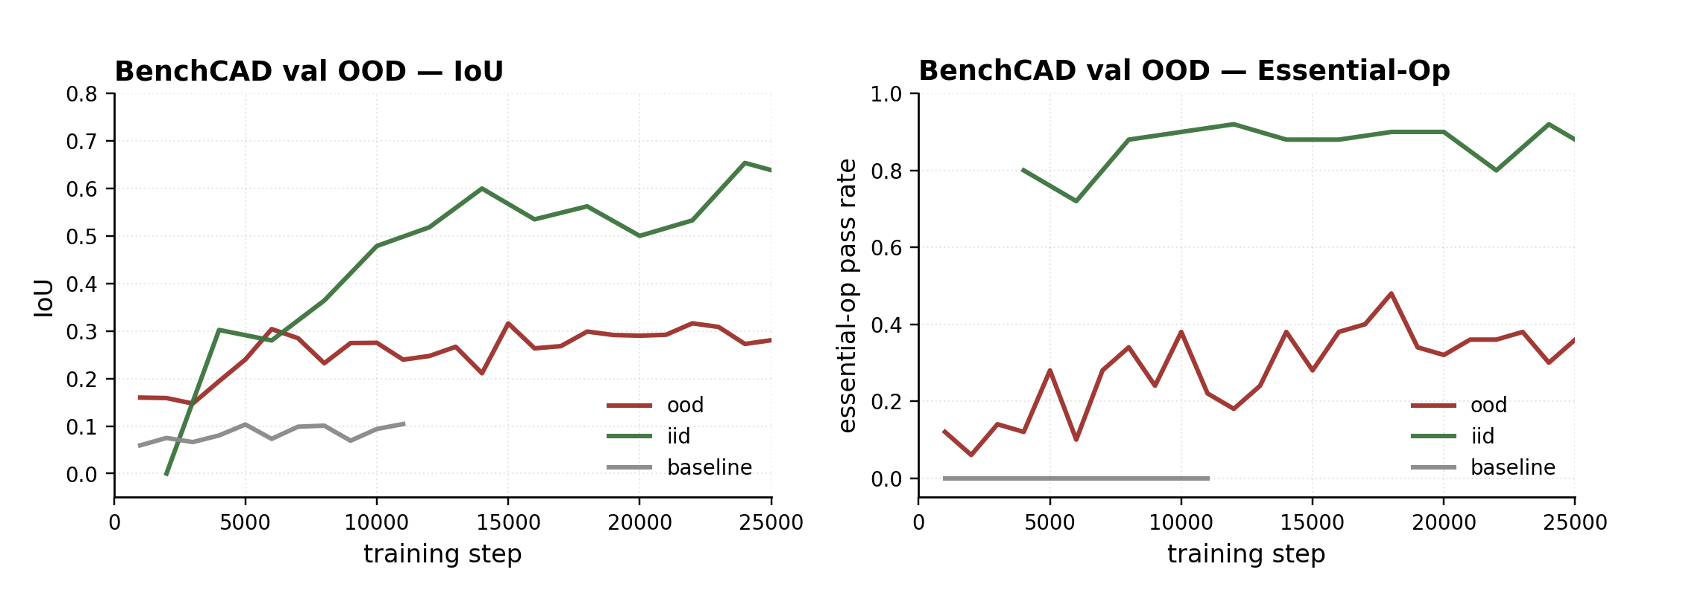
\includegraphics[width=0.85\linewidth]{figures/fig_7.png}
  \caption{\textbf{The generalisation gap on BenchCAD.} Qwen3-VL-2B trained on three data mixtures, evaluated on the BenchCAD validation set throughout training.
    \emph{(a) OOD IoU vs.\ training step.} The IID-trained run (green) climbs highest; the OOD run (red, trained without the held-out family slice) plateaus mid-range; the baseline (grey, no BenchCAD) stays near the floor.
    \emph{(b) OOD essential-op pass rate.} IID reaches the highest rate, OOD plateaus mid-range, baseline stays at $\sim$0\% --- the \textbf{CAD Operational Blindspot}.
    The deficit is not optimisation budget, not backbone capacity, and not training-corpus operation coverage alone --- it is the fundamental difficulty of constructing industry-grade parametric CAD code on \emph{unseen} family distributions.}
  \label{fig:generalisation_gap}
\end{figure*}
\section{Datasheet for BenchCAD}
\label{app:datasheet}

We follow the datasheet template of Gebru et al.\ (2021); responses below are condensed for the appendix and reproduced in full as a separate Croissant 1.0 metadata file shipped with the dataset release.

\paragraph{Motivation.}
\textbf{For what purpose was the dataset created?} BenchCAD was created to evaluate the parametric-CAD capabilities of large vision-language and code-language models along three sub-capabilities (visual perception, parametric abstraction, code synthesis) on industrially representative part families with execution-verified ground truth.
\textbf{Who created the dataset and on behalf of which entity?} The authors. (Anonymised for double-blind submission.)
\textbf{Who funded the dataset?} The authors' individual funds. (Anonymised.)

\paragraph{Composition.}
\textbf{What do the instances represent?} Each instance is a parametric CAD part: an executable CadQuery Python program, the resulting STEP file, four canonical-view PNG renders, a parameter JSON, and an op-list JSON.
\textbf{How many instances are there in total?} 17{,}900 verified parts in BenchCAD, 2{,}400 paired QA questions in BenchCAD-QA (each evaluated under both visual and code conditioning, yielding 4{,}800 records), and 748 curated edit pairs in BenchCAD-Edit.
\textbf{Does the dataset contain all possible instances?} No --- BenchCAD samples a subset of all the industry CAD generation part familys, and sampled a subset of parameter space per family; the schema permits unbounded sampling under the documented constraints.
\textbf{Is there a label/target?} The CadQuery source code, STEP, parameters, and op list jointly serve as ground truth; for QA tasks, gold answers are derived deterministically from parameters; for edit tasks, target code and target STEP are paired with the original.

\paragraph{Collection process.}
\textbf{How was the data acquired?} Procedurally generated by the BenchCAD generation pipeline (\S\ref{sec:dataset}); the only human-in-the-loop component is edit-pair curation by the authors.
\textbf{Who was involved in data collection?} The authors.
\textbf{Were any ethical review processes conducted?} Not applicable; no human-subjects data.

\paragraph{Preprocessing/cleaning/labeling.}
\textbf{Was preprocessing/cleaning done?} Verification (sandbox execution + non-degenerate volume + 30\,s timeout, followed by domain-expert visual sign-off) is the sole filter applied to BenchCAD.
The Fusion360 and DeepCAD subsets undergo additional curation: parsing failures and parts whose reconstruction yields invalid geometry are excluded.
\textbf{Was the raw data saved?} Yes; the unverified pre-filter output is retained for analysis and is available on request.

\paragraph{Uses.}
\textbf{Has the dataset been used for any tasks already?} The five tasks defined in \S\ref{sec:tasks}.
\textbf{Is there anything that prevents responsible reuse?} The dataset contains no PII, no copyrighted source designs, and no safety-sensitive specifications.
The standard-anchored families reference public ISO/DIN/EN/ASME/IEC standard codes by number and name; we do not redistribute the standard documents themselves.

\paragraph{Distribution.}
\textbf{Will the dataset be distributed?} Yes, on Hugging Face under \texttt{BenchCAD/cad\_bench} and \texttt{BenchCAD/cad\_bench\_edit}.
\textbf{When?} On submission acceptance (or on arXiv release if earlier).
\textbf{Under what licence?} CC-BY-4.0 for data; MIT for code (generation pipeline, evaluation harness, baseline checkpoint).
\textbf{Are there restrictions?} Standard CC-BY-4.0 attribution.

\paragraph{Maintenance.}
\textbf{Who will support the dataset?} The authors via the GitHub issue tracker and Hugging Face dataset card.
\textbf{How will errata be communicated?} Versioned releases on Hugging Face with changelogs in the dataset card.

\section{Question Bank Construction}
\label{app:qbank}

The numeric-QA tasks (\texttt{qa\_img}, \texttt{qa\_code}) draw from a per-family question bank constructed in three steps. (1) For each family, a domain-knowledge author writes 6--12 question \emph{templates} parameterised by the family's exposed parameters --- e.g.\ for \texttt{involute\_gear}: \emph{``what is the ratio of root-to-tip diameter?''}, \emph{``how many teeth does the visible gear have?''}.
Templates are typed (ratio, integer count, ordinal) and constrained to be scale-invariant. (2) Templates are instantiated per-record by deterministic substitution of the verified parameter values, yielding a gold answer alongside each question. (3) A second author reviews each instantiation for ambiguity and visibility (a question must be answerable from the four canonical views with no occluded features).
The final bank contains 2{,}400 unique (question, gold answer) pairs sampled across 17{,}900 records --- each evaluated under both visual (\texttt{qa\_img}) and code (\texttt{qa\_code}) conditioning, yielding 4{,}800 total QA records.
The composition is approximately 60\% ratio, 35\% integer count, and 5\% ordinal. We release the question-template source code so that the bank can be regenerated under alternative parameter samples.

\section{QA System Prompts}
\label{app:qa-system-prompts}

To ensure reproducibility, we provide the exact system prompts used in our QA evaluation.
All models are evaluated with the same prompt template. The model is required to output
only a JSON array of numbers, which enables automatic numeric grading. For binary
questions, we encode ``yes'' as 1 and ``no'' as 0.

\subsection{Image-based QA System Prompt}
\label{app:qa-img-system-prompt}

\begin{tcolorbox}[
    title=\texttt{QA\_IMG\_SYSTEM\_PROMPT},
    colback=gray!4,
    colframe=gray!45,
    fonttitle=\bfseries,
    breakable,
    sharp corners,
    boxrule=0.5pt,
]
\small
You are an expert CAD engineer. You will be shown a
\texttt{DIAGONAL\_VIEW\_LAYOUT}. You will be given a list of numeric
questions about the part. Answer each with a single number.

\vspace{0.5em}
\textbf{Rules:}
\begin{itemize}
    \item Output ONLY a JSON array of numbers, one per question, in the same order.
    \item No text, no keys, no explanation. Just the array.
    \item For yes/no questions, use 1 for yes and 0 for no.
    \item For count questions, use an integer, e.g., 12, not ``twelve''.
    \item For ratio questions, use a decimal, e.g., 2.5.
    \item For dimensional questions, answer in whatever consistent unit the code uses;
    the scale is arbitrary and the grader compares numeric magnitude.
\end{itemize}

\textbf{Example input:}
\begin{verbatim}
["How many teeth?", "What is the module?"]
\end{verbatim}

\textbf{Example output:}
\begin{verbatim}
[20, 2.5]
\end{verbatim}
\end{tcolorbox}

\subsection{Code-based QA System Prompt}
\label{app:qa-code-system-prompt}

\begin{tcolorbox}[
    title=\texttt{QA\_CODE\_SYSTEM\_PROMPT},
    colback=gray!4,
    colframe=gray!45,
    fonttitle=\bfseries,
    breakable,
    sharp corners,
    boxrule=0.5pt,
]

\small
You are an expert CAD engineer. You will be shown CadQuery Python code for a
mechanical part. You will be given a list of numeric questions about the part
this code produces.

\vspace{0.5em}
\textbf{Rules:}
\begin{itemize}
    \item Output ONLY a JSON array of numbers, one per question, in the same order.
    \item No text, no keys, no explanation. Just the array.
    \item For yes/no questions, use 1 for yes and 0 for no.
    \item For count questions, use an integer, e.g., 12, not ``twelve''.
    \item For ratio questions, use a decimal, e.g., 2.5.
    \item For dimensional questions, answer using the same scale as the numeric
    literals in the code.
\end{itemize}

\textbf{Example input code:} The code creates a gear with 20 teeth and module 2.5.

\textbf{Example input questions:}
\begin{verbatim}
["How many teeth in the gear?", "What is the module?"]
\end{verbatim}

\textbf{Example output:}
\begin{verbatim}
[20, 2.5]
\end{verbatim}
\end{tcolorbox}

\section{Code Generation System Prompts}
\label{app:codegen-system-prompts}

To ensure reproducibility, we provide the exact prompts used for code generation.
The model is given a normalized four-view composite render of an industrial part and
is asked to generate executable CadQuery Python code. All generated code is evaluated
under the same execution protocol: \texttt{cadquery} is pre-imported as \texttt{cq},
and the final reconstructed solid must be stored in \texttt{result}.

\subsection{Primary Vision-to-CAD System Prompt}
\label{app:primary-vision-to-cad-system-prompt}

\begin{tcolorbox}[
    title=\texttt{SYSTEM\_PROMPT},
    colback=gray!4,
    colframe=gray!45,
    fonttitle=\bfseries,
    breakable,
    sharp corners,
    boxrule=0.5pt
]
\small
Generate CadQuery Python code from a \texttt{DIAGONAL\_VIEW\_LAYOUT}.

\vspace{0.5em}
Renders are normalized: bbox centered at \texttt{[0.5,0.5,0.5]}, longest side maps to \texttt{[0,1]}.
Match the orientation exactly---do not rotate or remap axes. World XYZ in your code must match world XYZ in the renders.

\begin{itemize}
    \item \texttt{cadquery} is pre-imported as \texttt{cq}; no imports, no \texttt{show\_object}.
    \item Store final solid in \texttt{result}.
    \item Output ONLY code, no explanation or markdown.
\end{itemize}
\end{tcolorbox}

\subsection{Vision-to-CAD User Prompt}
\label{app:vision-to-cad-user-prompt}

\begin{tcolorbox}[
    title=\texttt{USER\_PROMPT},
    colback=gray!4,
    colframe=gray!45,
    fonttitle=\bfseries,
    breakable,
    sharp corners,
    boxrule=0.5pt
]
\small
Generate CadQuery code to recreate this industrial part shown in the 4-view composite render.
\end{tcolorbox}

\subsection{Cadrille Baseline System Prompt}
\label{app:cadrille-system-prompt}

\begin{tcolorbox}[
    title=\texttt{CADRILLE\_SYSTEM\_PROMPT},
    colback=gray!4,
    colframe=gray!45,
    fonttitle=\bfseries,
    breakable,
    sharp corners,
    boxrule=0.5pt
]
\small
You are a CadQuery expert. Given a normalized \texttt{DIAGONAL\_VIEW\_LAYOUT}.

\vspace{0.5em}
Write CadQuery Python code that reproduces the geometry. Output ONLY Python code.
\end{tcolorbox}


% \section{QA System Prompt}
% \label{app:qa_img_sys_prompt}

% \paragraph{QA\_IMG\_SYSTEM\_PROMPT}

% You are an expert CAD engineer. You will be shown a DIAGONAL\_VIEW\_LAYOUT. You will be given a list of numeric questions about the part. Answer each with a single number.

% Rules:\\
% - Output ONLY a JSON array of numbers, one per question, in the same order.\\
% - No text, no keys, no explanation. Just the array.\\
% - For yes/no questions, use 1 for yes and 0 for no.\\
% - For count questions, use an integer (e.g. 12, not "twelve").\\
% - For ratio questions, use a decimal (e.g. 2.5).\\
% - For dimensional questions, answer in whatever consistent unit the code uses (scale is arbitrary; the grader compares numeric magnitude).

% Example input: ["How many teeth?", "What is the module?"]\\
% Example output: [20, 2.5]

% \paragraph{QA\_CODE\_SYSTEM\_PROMPT}
% You are an expert CAD engineer. You will be shown CadQuery Python code for a mechanical part. You will be given a list of numeric questions about the part this code produces.

% Rules:
% - Output ONLY a JSON array of numbers, one per question, in the same order.\\
% - No text, no keys, no explanation. Just the array.\\
% - For yes/no questions, use 1 for yes and 0 for no.\\
% - For count questions, use an integer (e.g. 12, not "twelve").\\
% - For ratio questions, use a decimal (e.g. 2.5).\\
% - For dimensional questions, answer using the same scale as the numeric literals in the code.

% Example input code creates a gear with 20 teeth and module 2.5.
% Example input questions: ["How many teeth?", "What is the module?"]\\
% Example output: [20, 2.5]

\subsection{Edit-task System Prompt}
\label{app:edit-code-system-prompt}
\begin{tcolorbox}[title=\texttt{EDIT\_CODE\_SYSTEM\_PROMPT}, colback=gray!4, colframe=gray!45,fonttitle=\bfseries, breakable, sharp corners, boxrule=0.5pt,]                                   
  \small                                                         
  You are an expert CAD engineer. You will be given:
  \begin{enumerate}                                                   \item A CadQuery Python script that builds a parametric mechanical part.
      \item A natural-language edit instruction describing a change to one specific feature.                
  \end{enumerate}
    
  Your task: return the script with the MINIMAL edit that achieves the requested feature change. Only the feature(s) the instruction explicitly mentions should change; every other feature, dimension, and detail must stay exactly as in the original.    
  \vspace{0.5em}                                                  \textbf{Rules:}
  \begin{itemize}
  \item Output ONLY executable Python code, no explanation, no markdown fences.
  \item Make the smallest set of changes that realize the instruction. Do NOT touch unrelated literals, operations, or structure.
  \item Do NOT refactor, rename variables, reorder operations, or add/remove imports.
  \item If the instruction adds a new feature: append the operation in the most natural place; keep the rest of the chain intact.
  \item If the instruction removes a feature: delete just that operation block; do not rewrite surrounding code.
  \item If the instruction modifies a dimension/parameter: update only the literal(s) that depend on it (and, if present, the matching parameter comment).
  \end{itemize}
  \end{tcolorbox}                                                 
  
\label{app:edit-img-gt-system-prompt}                             \begin{tcolorbox}[
title=\texttt{EDIT\_IMG\_GT\_SYSTEM\_PROMPT},               
colback=gray!4, colframe=gray!45, fonttitle=\bfseries, breakable, sharp corners, boxrule=0.5pt,]
  \small
  You are an expert CAD engineer. You will be given:              
  \begin{enumerate}
  \item A CadQuery Python script that builds a parametric mechanical part(CURRENT state).
  \item A 2$\times$2 composite image of the TARGET geometry from 4 diagonal viewpoints.                                         
  \end{enumerate}                                                
  Your task: return the script with the MINIMAL edit that transforms the CURRENT geometry (described by the code) into the TARGET geometry (shown in the image). The image is the only specification of the desired change, there is NO text instruction. Compare the code's geometry against the image and infer which single feature differs.                      
  Only the feature(s) that differ between code and image should change; every other feature, dimension, and detail must stay exactly as in the original code.
    
  \vspace{0.5em}
  \textbf{Rules:}                                                               
  \begin{itemize}
  \item Output ONLY executable Python code, no explanation, no markdown fences.
  \item Make the smallest set of changes that realize the visual difference. Do NOT touch unrelated literals, operations, or structure.
  \item Do NOT refactor, rename variables, reorder operations, or add/remove imports.
  \item If the target image shows a new feature that is absent in the code: append the operation in the most natural place; keep the rest of the chain intact.
  \item If the target image shows a feature removed: delete just that operation block; do not rewrite surrounding code.
  \item If a dimension/parameter has changed: update only the literal(s) that control that dimension (and the matching parameter comment if present).  
  \end{itemize}
  \end{tcolorbox} 



\label{app:edit-img-system-prompt}

\begin{tcolorbox}[
    title=\texttt{EDIT\_CODE\_IMG\_SYSTEM\_PROMPT (Ablation)},
    colback=gray!4,
    colframe=gray!45,
    fonttitle=\bfseries,
    breakable,
    sharp corners,
    boxrule=0.5pt,
]
\small
You are an expert CAD engineer. You will be given:
\begin{enumerate}
    \item A CadQuery Python script that builds a parametric mechanical part.
    \item A natural-language edit instruction describing a change to one specific feature.
    \item A 2$\times$2 composite image of the part from 4 diagonal viewpoints (CURRENT state) as an additional visual reference for the script.
\end{enumerate}

Your task: return the script with the MINIMAL edit that achieves the
requested feature change. Only the feature(s) the instruction explicitly
mentions should change; every other feature, dimension, and detail must
stay exactly as in the original.

\vspace{0.5em}
\textbf{Rules:}
\begin{itemize}
    \item Output ONLY executable Python code, no explanation, no markdown fences.
    \item Make the smallest set of changes that realize the instruction. Do NOT touch unrelated literals, operations, or structure.
    \item Do NOT refactor, rename variables, reorder operations, or add/remove imports.
    \item If the instruction adds a new feature: append the operation in the most natural place; keep the rest of the chain intact.
    \item If the instruction removes a feature: delete just that operation block; do not rewrite surrounding code.
    \item If the instruction modifies a dimension/parameter: update only the literal(s) that depend on it (and, if present, the matching parameter comment).
\end{itemize}
\end{tcolorbox}




\section{Rotation-Invariant IoU}
\label{app:iou}

We compute IoU under a configurable rotation-invariant protocol, taking the maximum over either the 6-element face-up cube symmetry group or the full 24-element cube rotation group. Before voxelization, each part is normalized by centering it at the origin and scaling it by the largest semi-axis of its bounding box. For each candidate rotation $g \in G$, we rotate the predicted voxel grid $\hat{V}$ and compute its overlap with the reference voxel grid $V$; the reported score is
\[
\max_{g \in G} \mathrm{IoU}(g \cdot \hat{V}, V).
\]
This metric is used diagnostically rather than as the primary score: a large gain from standard IoU to 24-rotation IoU indicates that the model may have generated the right geometry on the wrong construction plane. This failure is partly induced by a workplane prior: in online database, and manufacturing-oriented modeling workflows, parts are commonly initialized on the \texttt{XY} plane as the default sketching or setup plane. As a result, models may over-prefer \texttt{XY}-based constructions even when the target geometry is defined on \texttt{XZ} or \texttt{YZ}. Consistent with this interpretation, Table~\ref{tab:rot24_base_plane} shows substantially larger rotation-IoU gains for \texttt{XZ}/\texttt{YZ} ground-truth parts than for \texttt{XY} parts.
\begin{table}[t]
\centering
\small
\setlength{\tabcolsep}{6pt}
\renewcommand{\arraystretch}{1.08}
\caption{\textbf{Effect of rotation-invariant IoU by GT base plane.}
For GPT-4o, we report $\Delta=\mathrm{IoU}_{\mathrm{rot24}}-\mathrm{IoU}_{\mathrm{single\text{-}axis}}$ over 164 valid 24-IoU samples with extrusion. Larger $\Delta$ indicates cases where the generated shape is geometrically similar but expressed in a mismatched coordinate frame.}
\label{tab:rot24_base_plane}
\begin{tabular}{@{}lrrrr@{}}
\toprule
GT base plane & $n$ & Mean $\Delta$ & Max $\Delta$ \\
\midrule
XY  & 70  & 0.0463 & 0.5907 \\
XZ  & 40  & 0.2305 & 0.8031 \\
YZ  & 54  & 0.2140 & 0.7053 \\
\bottomrule
\end{tabular}
\end{table}

\section{Edit Protocol}
\label{app:edit_protocol}

\paragraph{Pair construction.} The 748 BenchCAD-Edit pairs are drawn balanced across 106 families and four edit categories (balanced across dimensional, additive, subtractive, and multi-step categories).
For each pair, we (i) start from a verified BenchCAD record, (ii) apply a parameter or op-list edit yielding a target part, (iii) verify the target satisfies the same verification pipeline, (iv) write a natural-language instruction by template (\emph{``increase the bore diameter to 12\,mm''}) reviewed for unambiguity by a second author, and (v) cross-validate by running two strong models and inspecting any unexpected failure modes.
Pairs where models systematically disagree on instruction interpretation are revised or removed.

\paragraph{Scoring.} See Eq.~\ref{eq:edit_acc} for metric definitions (normalised IoU used in edit-task score). The non-target preservation check is computed on the spatial complement of the bounding region of the targeted feature (precomputed bounding-box annotation per pair).


\paragraph{Task taxonomy.} The five edit task types (T1--T5) are defined in Table~\ref{tab:task_taxonomy}. Difficulty rises monotonically with the structural complexity of the minimal correct diff, from a single literal swap (T1) to coordinated multi-block restructures (T5). The T1--T5 axis is orthogonal to the dimensional/additive/subtractive/multi-step categorisation used in the main paper: T1 and T3 are predominantly dimensional, T2 and T4 cover additive/subtractive, and T5 spans the multi-step regime.

\begin{table}[t]
\centering
\caption{\textbf{BenchCAD-Edit task taxonomy.} The 748 edit pairs are stratified into five task types T1--T5 by the structural form of the minimal correct diff. Difficulty rises monotonically from T1 (one-literal swap) to T5 (multi-block restructure with trig or coordinated sub-feature changes).}
\label{tab:task_taxonomy}
\small
\begin{tabular}{@{}p{0.04\linewidth}p{0.18\linewidth}p{0.30\linewidth}p{0.18\linewidth}p{0.20\linewidth}@{}}
\toprule
\textbf{Code} & \textbf{Name} & \textbf{Definition} & \textbf{Diff signature} & \textbf{Example instruction} \\
\midrule
T1 & literal\_replace & Replace a single numeric literal that the instruction names explicitly (\emph{from X to Y}). & one literal swap; equal lines added/removed & \emph{``Increase the cylinder radius from 4.5 to 5.85.''} \\
T2 & chain\_transform & Append a single chainable whole-part transform (rotate / mirror / array). & one \texttt{result = result.<op>(...)} line appended & \emph{``Rotate the entire part by 90 degrees about the X axis.''} \\
T3 & relative\_compute & Read an existing literal and derive another value (ratio, percentage, $2\times$, $1/4$). & one literal swap, value derived from another literal & \emph{``Set the central bore diameter equal to twice the hub-cylinder height.''} \\
T4 & feature\_edit & Add or delete a single CSG sub-block (hole, slot, recess, chamfer, fillet, boss). & one 3--7 line CSG block inserted or removed & \emph{``Drill a 6 diameter through-hole along the Z axis.''} \\
T5 & geometry\_rebuild & Non-trivial restructure: trig-derived slopes/chamfers/lofts, or paragraph-style rebuilds where two or more sub-features change in concert. & multi-block rewrite, trig in code, paragraph instruction & \emph{``Replace the ramped arms and raised center with a single flat cross-shaped solid of uniform thickness.''} \\
\bottomrule
\end{tabular}
\end{table}



\paragraph{Failure taxonomy.} Every failing prediction is bucketed into one of eight semantic failure modes F01--F08 (Table~\ref{tab:failure_codes}), each mapped to one of the four capability layers L1--L4: F01--F03 isolate L1 \emph{Holistic Visual Understanding} (wrong value, wrong instance, wrong placement), F04--F06 isolate L2 \emph{CAD Operations Comprehension} (wrong axis, wrong selector, near no-op), F07 isolates L3 \emph{Industrial Parametric Abstraction} (incomplete multi-instance update), and F08 isolates L4 \emph{Spatial Reasoning $+$ Code Synthesis} (compositional geometry mismatch). Each label combines an automatic detection cue --- execution status, generated-vs-original/target IoU thresholds, and topology checks with a hand audit by the authors against the predicted code and rendered geometry; the rule set and L-mapping are fixed across all ten models reported, and \texttt{ok} (strict pass) and \texttt{exec\_fail} are tracked separately as the non-failure and gross-execution categories.

\begin{table}[t]
\centering
\caption{\textbf{Failure-mode taxonomy (F-codes).} Eight semantic failure modes used in the per-model failure analysis (Fig.~\ref{fig:edit_F_bars}). Each F-code is mapped to one capability layer: L1 \emph{Holistic Visual Understanding}, L2 \emph{CAD Operations Comprehension}, L3 \emph{Industrial Parametric Abstraction}, L4 \emph{Spatial Reasoning $+$ Code Synthesis}. Hand-labelled on the failing predictions of every BenchCAD-Edit run.}
\label{tab:failure_codes}
\small
\setlength{\tabcolsep}{4pt}
\renewcommand{\arraystretch}{1.15}
% allow line breaks at underscores in fixed-width name cells
\newcommand{\fname}[1]{\seqsplitfallback{#1}}
\providecommand{\seqsplitfallback}[1]{#1}
\begin{tabular}{@{}p{0.06\linewidth}p{0.18\linewidth}p{0.28\linewidth}p{0.18\linewidth}p{0.18\linewidth}@{}}
\toprule
\textbf{Code} & \textbf{Name} & \textbf{Definition} & \textbf{Detection cue} & \textbf{Representative failure} \\
\midrule
F01 \mbox{(L1)} & wrong\_\allowbreak param\_\allowbreak value & Right operation, wrong numerical value: dim, diameter, radius, length, or angle written off-target; geometry shape-correct but a single number misses. & $\mathrm{IoU}_{\text{gen}} \geq 0.9$, output differs from target by a single literal. & Model writes radius $5.6$ when prompt asks for $5.85$; cylinder topology unchanged. \\
F02 \mbox{(L1)} & wrong\_\allowbreak feature\_\allowbreak instance & Among multiple similar features (front vs.\ back ring, two legs, several circles), the model edits the wrong one or perturbs a neighbour. & $\mathrm{IoU}_{\text{gen}}$ swings markedly above OR below baseline; topology preserved. & Edit asks to enlarge the rear bore; model enlarges the front bore. \\
F03 \mbox{(L1)} & wrong\_\allowbreak placement & Right operation and value, but feature placed at slightly wrong coordinate, face, or orientation. & $\mathrm{IoU}_{\text{gen}} \geq 0.95$, small rigid offset against target. & Hole drilled $2$\,mm off-centre on a face whose origin the model misread. \\
F04 \mbox{(L2)} & wrong\_\allowbreak axis\_\allowbreak or\_\allowbreak direction & Rotation, mirror, or extrude direction wrong: rotate axis tuple permuted, mirror plane misidentified, sweep tangent flipped. & \texttt{status==ok}; rotated/mirrored bbox mismatches target axis. & gpt-4o rotate: \texttt{rotate((axis), (origin), deg)} with first two args swapped. \\
F05 \mbox{(L2)} & wrong\_\allowbreak selector\_\allowbreak or\_\allowbreak face & \texttt{.faces()}/\texttt{.edges()} selector returns wrong subset: \texttt{>Y} chosen on a Z-up part, OR-selector returns multi-face, lofted-face selector silently misses. & \texttt{status==ok}; operation applied to wrong topology vs.\ target. & Chamfer applied to all top edges instead of the single outer rim. \\
F06 \mbox{(L2)} & near\_\allowbreak no\_\allowbreak op\_\allowbreak under\_\allowbreak edit & Output $\approx$ original: comment-only edit, deleted wrong line, retained the feature meant to be removed, or applied the edit with no observable geometric effect. & $|\mathrm{IoU}_{\text{gen}} - \mathrm{IoU}_{\text{orig}}| < 0.005$. & claude-opus-4-7 (no-think): on $49\%$ of the failed records that rewrites the original byte-for-byte. \\
F07 \mbox{(L3)} & incomplete\_\allowbreak multi\_\allowbreak update & Edit requires updating multiple symmetric or repeated instances (helical-sweep points, replicated bolts/legs); model updates only a subset. & $\mathrm{IoU}_{\text{gen}}$ plateaus below $1.0$ across attempts; partial symmetry break. & Cross-parameter dim asks to scale all four legs; model scales only two. \\
F08 \mbox{(L4)} & compositional\_\allowbreak geometry\_\allowbreak mismatch & Composite or structural shape (slope strip, loft, sweep cross-section, multi-feature reorganisation) is partially right but does not match GT topology. & \texttt{status==ok}; $\mathrm{IoU}_{\text{gen}} \in [0.4, 0.95]$ on a T5-style edit. & Slope edit produces a chamfer of correct angle but along the wrong face strip. \\
\bottomrule
\end{tabular}
\end{table}



\paragraph{Image-conditioned variant.} To probe whether the textual instruction itself is a confound --- i.e.\ whether models succeed because the instruction states the change explicitly rather than because they reason about the geometry --- we additionally evaluate an image-conditioned setting in which the natural-language instruction is replaced by a four-view render of the target solid (\texttt{EDIT\_IMG\_GT\_SYSTEM\_PROMPT}, Appendix~\ref{app:edit-img-gt-system-prompt}); the model receives the original code and must infer the edit visually. Across the four OpenAI models we tested, \texttt{mean\_norm} drops by $0.40$--$0.85$\,pt at every task type (Fig.~\ref{fig:edit_image_type}). The dominant failure mode is that a render specifies geometry but not numbers: the model can usually tell whether a feature is added or removed (T2/T4 retain weak signal), but cannot recover the exact dimension a textual ``from $X$ to $Y$'' would have stated, so dimensional edits (T1, T3) collapse to near-zero and trig-driven rebuilds (T5) floor uniformly at $0$. Image-only conditioning is therefore a strict lower bound on the text protocol and, in its current form, primarily isolates feature-presence reasoning rather than parametric exactness.

                                               

\paragraph{Supplementary results.} Figure~\ref{fig:edit_F_bars} reports failure attributes of all 748 eidt-pairs from 10 LLMs.
Figure~\ref{fig:edit_L_pies} disaggregates per-model failures into the L1--L4 buckets defined in Figure~\ref{fig:capability_hierarchy}. Figure~\ref{fig:edit_image_type} reports the parallel image-based setting (target render in lieu of an NL instruction) broken down by T1--T5.

\begin{figure}[t]                       
    \centering
    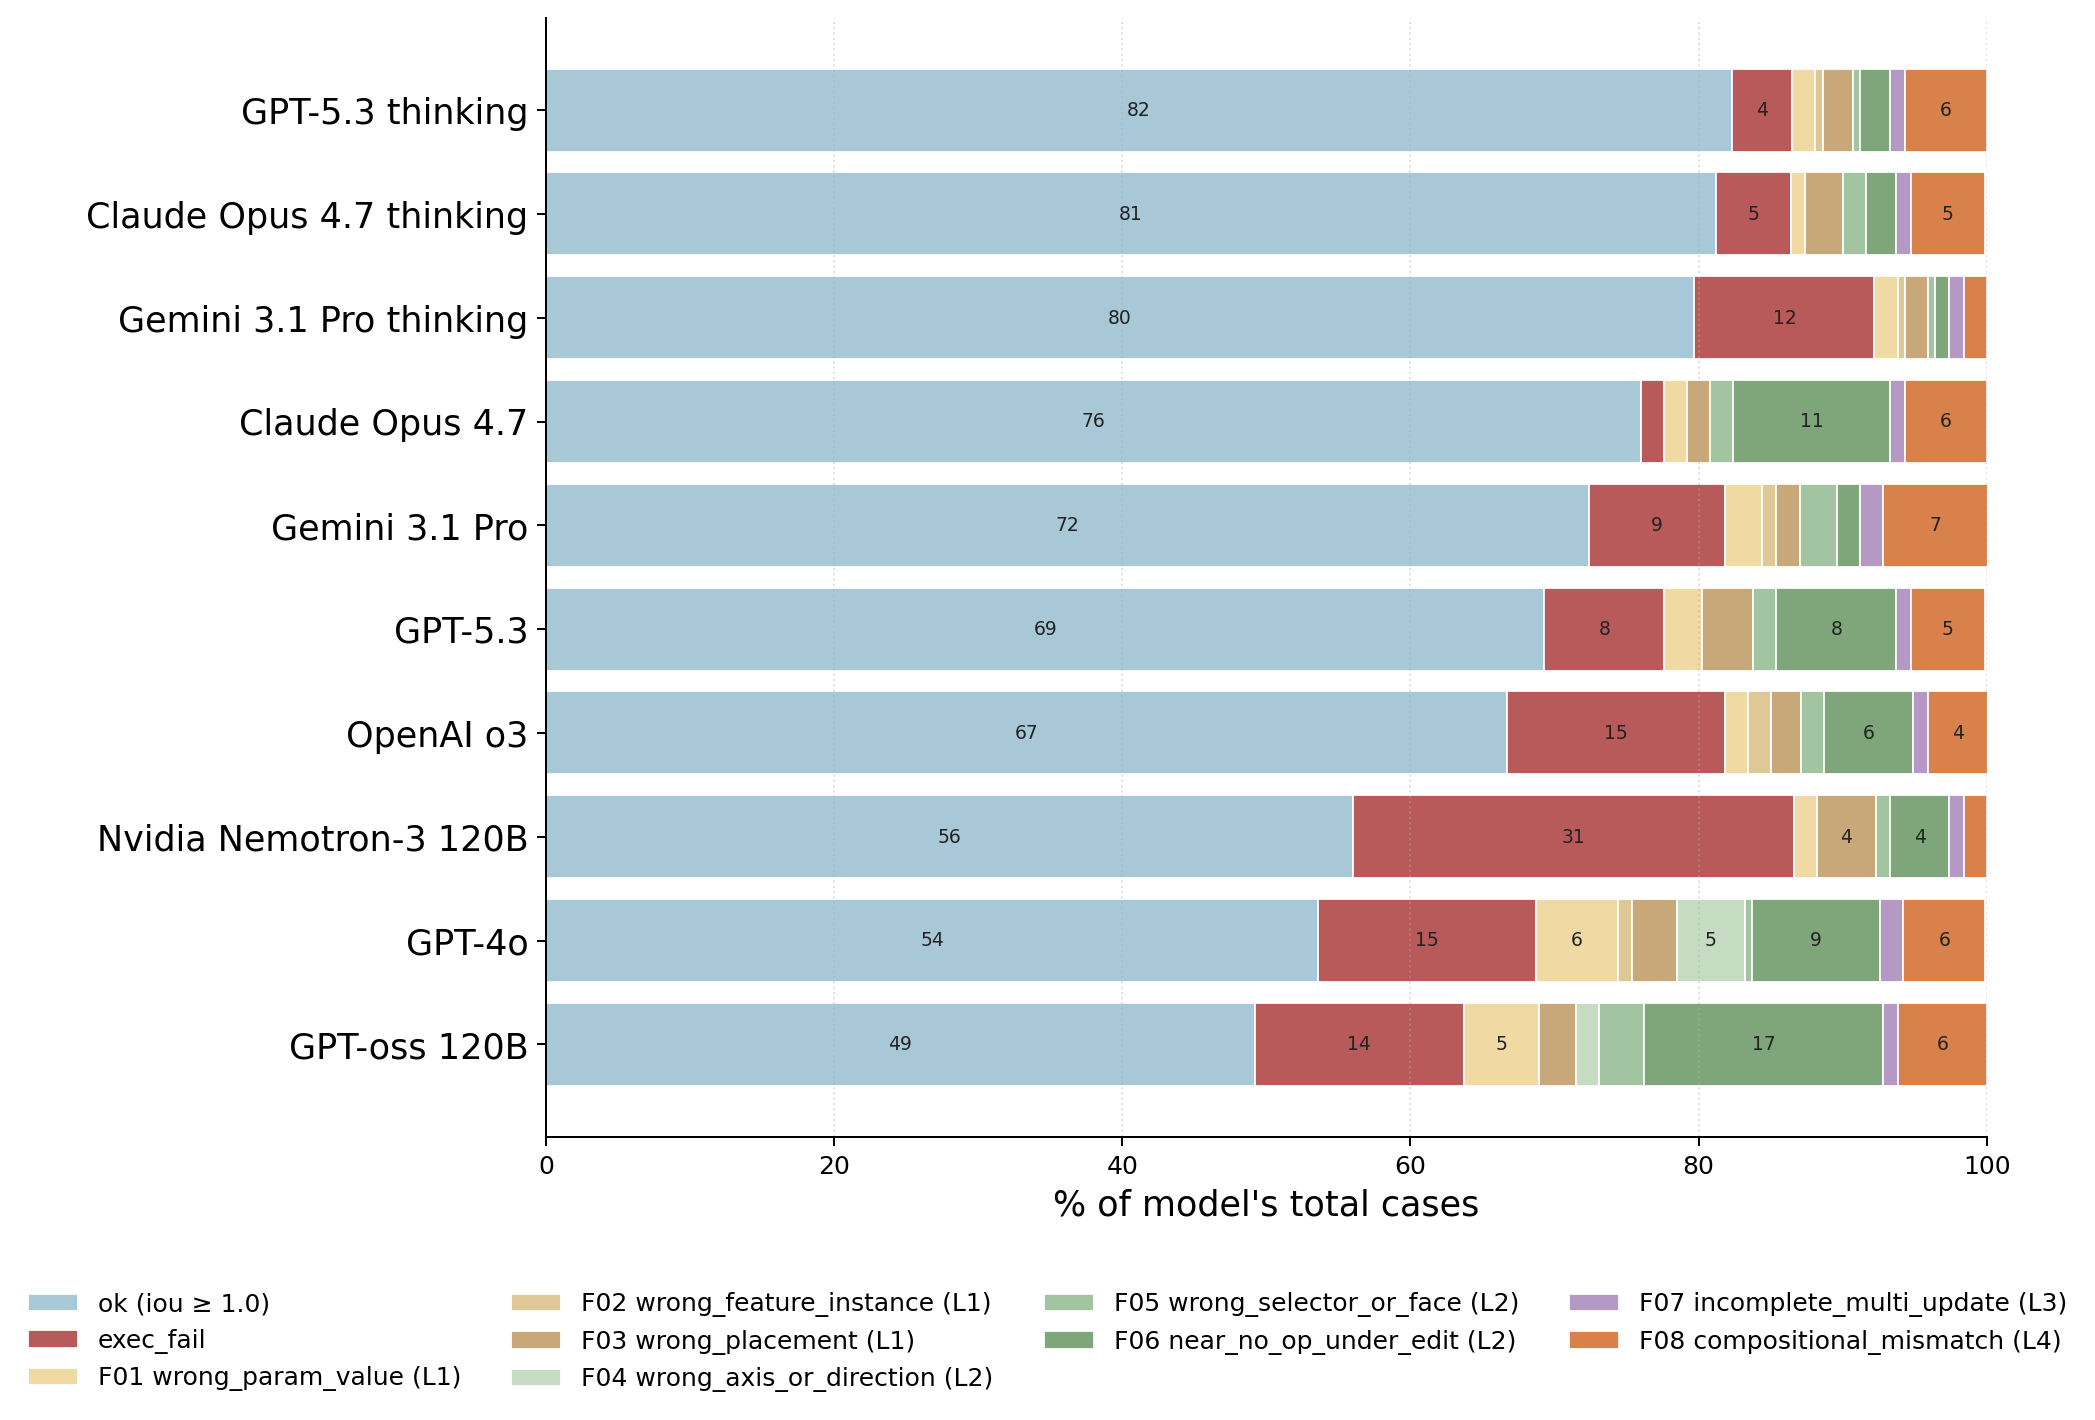
\includegraphics[width=0.95\linewidth]{figures/fig_F_bars.png}
    \caption{\textbf{Per-model failure-mode distribution on BenchCAD-Edit.} Each
   horizontal bar disaggregates one model's predictions into \texttt{ok},
  \texttt{exec\_fail}, and the eight semantic failure modes F01--F08 defined in 
  Table~\ref{tab:failure_codes}; segments are coloured by the underlying
  capability layer (sand $=$ L1 \emph{Holistic Visual Understanding}, sage $=$  
  L2 \emph{CAD Operations Comprehension}, purple $=$ L3 \emph{Industrial
  Parametric Abstraction}, orange $=$ L4 \emph{Spatial Reasoning $+$ Code       
  Synthesis}), so the L-mass within each bar reads off directly. Models are
  ordered by \texttt{ok} rate. The mass shifts systematically across model    
  generations: older or smaller-capacity systems concentrate failures in the L2
  band (F04--F06) and incur a non-trivial \texttt{exec\_fail} tail; recent large
   models without explicit reasoning largely close the L2 gap and leave residual
   mass on L1 (F01--F03); reasoning-tier closed models flatten L1 and L2 alike
  but expose an L3--L4 ceiling (F07--F08) on multi-instance and T5-style
  coordinated edits, indicating that thinking lifts capability up the
  L-hierarchy rather than uniformly reducing all error types.}
    \label{fig:edit_F_bars}
  \end{figure}  

\begin{figure}[t]
  \centering
  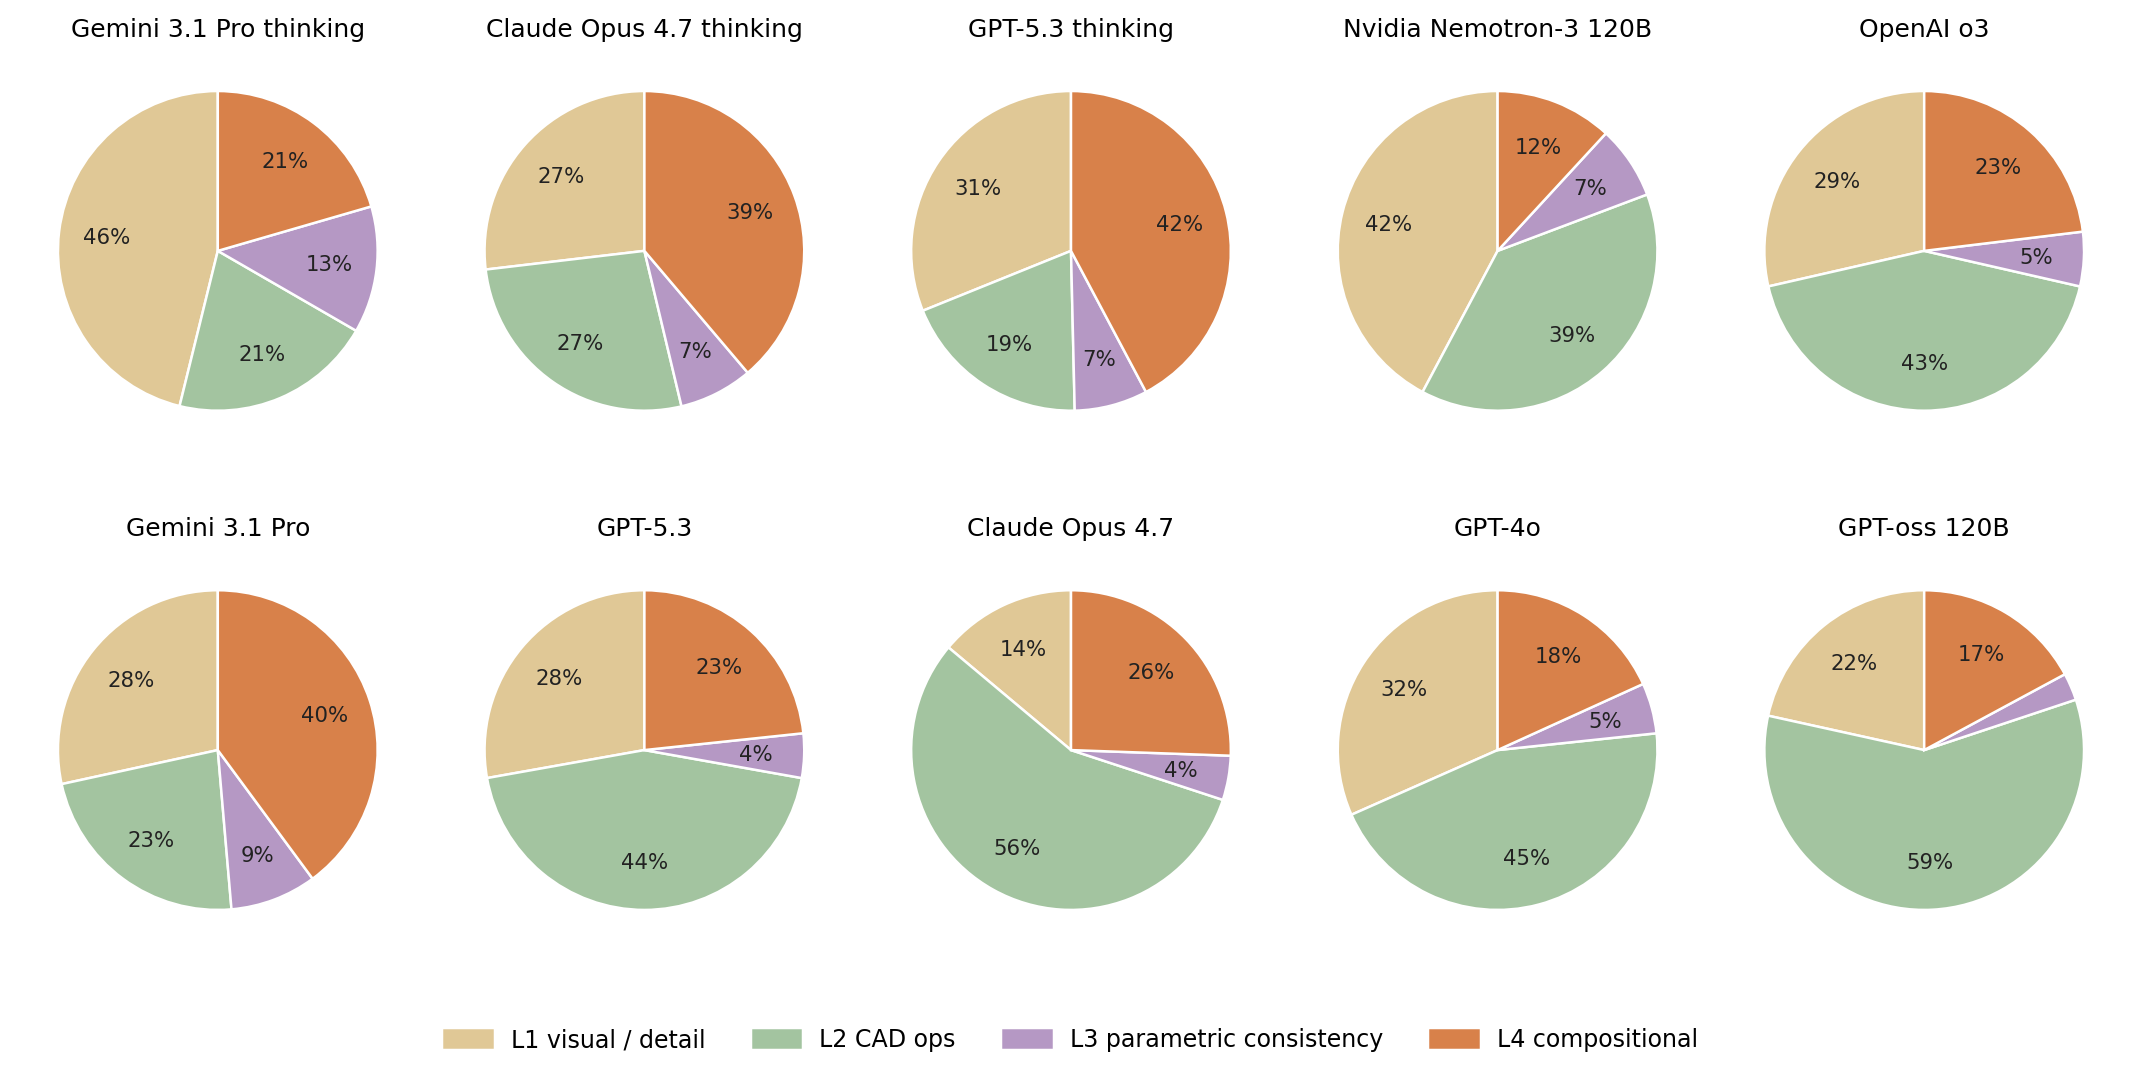
\includegraphics[width=0.95\linewidth]{figures/fig_L_pies.png}
  \caption{\textbf{Per-model failure-layer distribution on BenchCAD-Edit.} Each pie shows one model's failures aggregated by capability layer L1--L4 (collapsing the eight F-codes via the mapping in Table~\ref{tab:failure_codes}: F01--F03 $\to$ L1, F04--F06 $\to$ L2, F07 $\to$ L3, F08 $\to$ L4) and re-normalised so L1$+$L2$+$L3$+$L4 $= 100\%$ --- i.e.\ the pies show the \emph{shape} of each model's failure mode mix, independent of how often it fails overall; the title above each pie reports the absolute L-fail rate (\% of all predictions) so that scale is preserved. Models are arranged in order of increasing total L-fail rate (least-broken first). The mass shifts systematically along the L-axis across model generations: older or smaller-capacity systems concentrate failures in L2 (CAD-API misuse) and incur a non-trivial \texttt{exec\_fail} tail (counted separately, not shown); recent large models without explicit reasoning largely close the L2 gap and leave residual mass on L1 (visual/detail mistakes); reasoning-tier closed models flatten L1 and L2 alike but expose an L3--L4 ceiling on multi-instance and T5-style coordinated edits, indicating that thinking lifts capability up the L-hierarchy rather than uniformly reducing all error types.}
  \label{fig:edit_L_pies}
\end{figure}

\begin{figure}[t]
  \centering
  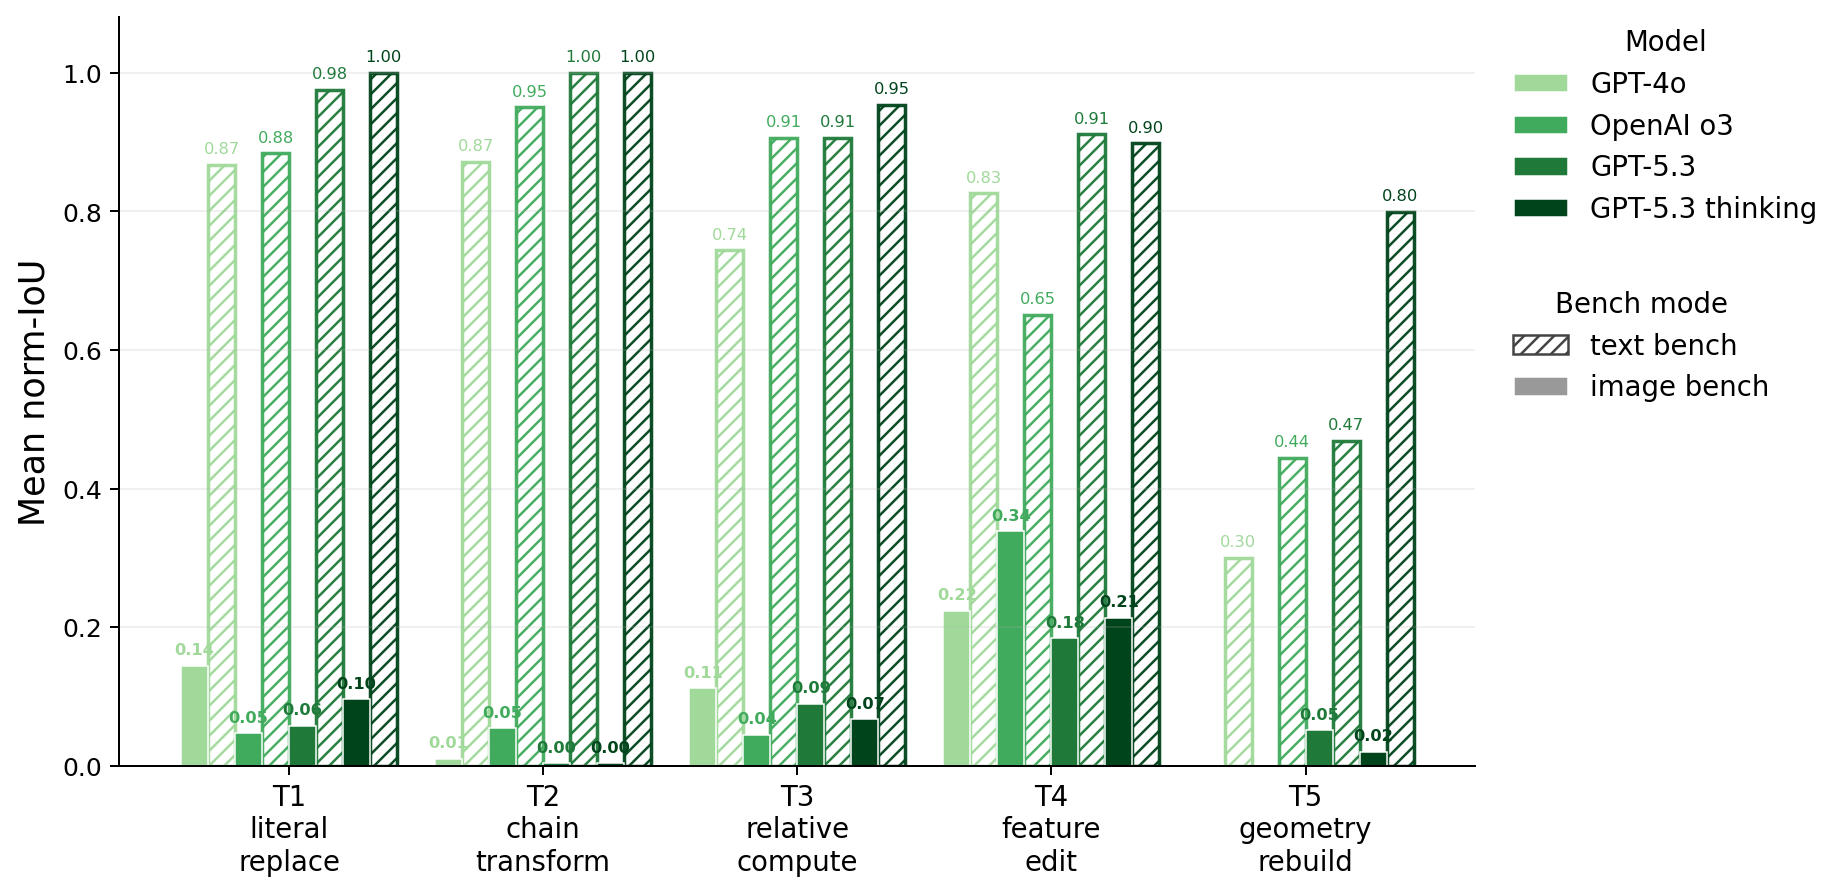
\includegraphics[width=0.95\linewidth]{neurips_2026/figures/fig_edit_image_type.png}
  \caption{\textbf{Text vs.\ image conditioning.} Same $100$-pair subset, four OpenAI models, two protocols: \emph{text} sees the original code plus a natural-language instruction, \emph{image} replaces the instruction with a four-view render of the target solid (\texttt{EDIT\_IMG\_GT\_SYSTEM\_PROMPT}, App.~\ref{app:edit-img-gt-system-prompt}). Bars are \texttt{mean\_norm} (Eq.~\eqref{eq:edit_acc}) per task type. Text dominates uniformly, with the largest gaps at T1 and T3: a render shows what the part should look like but never tells the model that a radius is $5.85$, so dimensional edits collapse. T2 and T4 retain weak image signal because adding or removing a feature is something a render can communicate. T5 floors at zero either way. Reasoning helps the text side substantially but barely moves the image side, so current chain-of-thought mostly strengthens code-side reasoning rather than visual diff inference. Image-only conditioning is a strict lower bound on the text protocol; in its current form it primarily probes feature-presence reasoning, not parametric exactness.}
  \label{fig:edit_image_type}
\end{figure}


\section{Scoring-Protocol Ablations}
\label{app:ablation}

\begin{table}[t]
\centering
\small
\caption{\textbf{Scoring-protocol and inference-strategy ablations.} Reported on GPT-5.3 (think) on BenchCAD-Lite. Removing scale invariance (allowing absolute mm hints in prompts) inflates \texttt{qa\_img} by 4.6\,pt --- the systematic optimism baked into prior CAD-eval protocols. Best-of-5 sampling and multi-turn refinement with execution feedback offer diminishing-returns improvements. Doubling view count from 4 to 8 closes only $\leq$1.5\,pt of the Holistic Spatial and Detailing Deficit, far below what a perception bottleneck would predict.}
\label{tab:ablation}
\begin{tabular}{lrr}
\toprule
Variant & Avg & $\Delta$ \\
\midrule
GPT-5.3 full (4-view img + scale-invariant prompts) & 46.8 & -- \\
$-$ single front view only                        & 38.5 & $-$8.3 \\
$+$ 8-view grid (vs.\ 4-view)                     & 47.6 & $+$0.8 \\
$-$ scale-invariant prompts (mm hints leak)       & 51.4 & $+$4.6 (inflated) \\
$-$ rotation-invariant IoU (axis-aligned only)    & 40.9 & $-$5.9 (under-credited) \\
$+$ Best-of-5 sampling                            & 52.1 & $+$5.3 \\
$+$ multi-turn refinement w/ exec feedback (3 turns) & 55.8 & $+$9.0 \\
\bottomrule
\end{tabular}
\end{table}


Table~\ref{tab:ablation} reports two scoring-protocol ablations on the Vision2Code task. (i) The \emph{24-axial vs.\ single-axis IoU} contrast quantifies how much credit is recovered by accounting for wrong-plane outputs (\S\ref{sec:exp_failure_analysis}, $L_1$ spatial-anchoring failure mode): when the gap is large, the model's geometry is approximately correct but emitted on a non-canonical workplane. (ii) The \emph{single-view vs.\ multi-view} contrast quantifies how much of a model's score is driven by the four-view evidence specifically, isolating the cost of removing back-side and depth cues from the perception input.

\section{CadQuery Operation Coverage}
\label{app:ops}

\begin{table}[t]
\centering
\small
\caption{\textbf{CadQuery operation coverage versus prior corpora.} BenchCAD covers 28 distinct operations spanning primitives, 2D sketching, advanced solid ops (helical sweeps, lofts, shells), boolean composition, holes, arrays, and finishing features. Prior CAD datasets are largely restricted to sketch + extrude.}
\label{tab:op_coverage}
\begin{tabular}{lccccccc}
\toprule
Bench & sk+ex & rev. & loft/sw. & bool. & fil/cham & twistEx. & spline/helix \\
\midrule
DeepCAD              & \cmark & --     & --     & basic  & --     & --     & --     \\
Text2CAD             & \cmark & --     & --     & --     & --     & --     & --     \\
CAD-Coder            & \cmark & --     & --     & --     & --     & --     & --     \\
CAD-Recode (1M)      & \cmark & --     & --     & \cmark & --     & --     & --     \\
CADPrompt (200)      & \cmark & part.  & part.  & \cmark & --     & --     & --     \\
CADEvolve            & \cmark & \cmark & --     & \cmark & part.  & --     & --     \\
\midrule
\textbf{BenchCAD}    & \cmark & \cmark & \cmark & \cmark & \cmark & \cmark & \cmark \\
\bottomrule
\end{tabular}
\end{table}


Table~\ref{tab:op_coverage} reports the per-category breakdown.

\paragraph{Static analysis protocol.}
For each released CadQuery corpus we extract distinct method invocations using the regex \texttt{$\backslash$.([A-Za-z\_]\textbackslash w*)(} on the \texttt{.py} text. We then EXCLUDE three groups: (a) class/type names (\texttt{Workplane}, \texttt{Vector}, \texttt{Wire}, \texttt{Solid}, \texttt{Sketch}, \texttt{Compound}, \texttt{Edge}, \texttt{Face}, \texttt{Plane}, \texttt{Location}, \texttt{Shape}, \texttt{Edges}, \texttt{Vertices}); (b) selectors / accessors that do not modify geometry (\texttt{face}, \texttt{faces}, \texttt{edges}, \texttt{vertices}, \texttt{wires}, \texttt{val}, \texttt{vals}, \texttt{first}, \texttt{last}, \texttt{tag}, \texttt{newObject}, \texttt{copyWorkplane}, \texttt{plane}); and (c) Python stdlib / numpy / utility helpers (\texttt{append}, \texttt{join}, \texttt{format}, \texttt{sin}, \texttt{cos}, \texttt{multiply}, \ldots). The same EXCLUDE list is applied uniformly across BenchCAD, CADEvolve seeds, CAD-Recode/cadrille, GenCAD-Code, and CADPrompt. Saturation curves: CAD-Recode at $1{,}274$ \texttt{.py} (op count constant from $200$ files onward); GenCAD-Code at $2{,}000$ streamed samples (constant from $100$ samples onward).

\paragraph{Tier B (sketch+extrude IR works).}
DeepCAD, Fusion360 Gallery, and Text2CAD release a tokenized intermediate representation rather than executable CadQuery, so the CadQuery static-analysis rule does not apply directly. We instead report the IR's primitive-token alphabet: DeepCAD encodes parts as \{\texttt{L}, \texttt{A}, \texttt{C}, \texttt{EXT}\} plus two control tokens \{\texttt{SOL}, \texttt{EOS}\} (\citet{Wu2021}, Sec.~3); Fusion360 Gallery r1.0.1 specifies $8$ sketch curve types (\texttt{SketchLine}, \texttt{SketchArc}, \texttt{SketchCircle}, \texttt{ConicCurve}, \texttt{Ellipse}, \texttt{EllipticalArc}, \texttt{FittedSpline}, \texttt{FixedSpline}) plus extrude with $4$ boolean variants \citep{Willis2021fusion}; Text2CAD reuses the CAD-SIGNet tokenizer ($\sim$$17$-token alphabet over end-of-X markers, quantized coords, and $4$ extrude booleans). These counts are not directly comparable to method counts on CadQuery \texttt{.py} releases; in Table~\ref{tab:cmp_prior} we accordingly summarize each work as \emph{narrow} (sketch+extrude IR or a small CadQuery subset) or \emph{broad} (wide CadQuery API).

\paragraph{CADEvolve caveat.}
CADEvolve's Hugging Face release (\texttt{kulibinai/cadevolve}, $\sim$$2$M rows, $4.7$\,GB) contains only \texttt{.npy} sentence embeddings keyed by component name, not Python source. The full $\sim$$1.3$M expanded scripts are referenced in the paper but are not part of the public release. We therefore report CADEvolve's operation count from the $46$ hand-written seed programs in \texttt{evolution/cadquery\_examples.txt} of the GitHub repo \texttt{zhemdi/CADEvolve}, yielding $30$ distinct ops --- a strict lower bound on the full evolved corpus.

\section{Reproduction Recipe}
\label{app:reproduce}

Reproduction uses the released \texttt{bench/fetch\_data.py} (Hugging Face fetch), the \texttt{bench.eval} runner (\texttt{--model <model> --task <task> --seed 42}), and each released model's documented inference entry-point.
We provide adapter wrappers under \texttt{bench/models/providers/} for cadrille and CADEvolve so that the existing runner accepts these models without modification.
Per-task IoU, Chamfer distance, execution rate, and per-family breakdowns are exported to \texttt{results/<task>/<model>/}.
For training the open BenchCAD baseline: \texttt{train/sft\_qwen3vl.py} with the released training config and data manifest.

\clearpage
\section{Ethical Considerations and Broader Impact}
\label{app:ethics}

BenchCAD contains procedurally generated parametric CAD parts and references public engineering standards by code and name.
The dataset contains no personal data, no proprietary designs, and no safety-sensitive specifications.
Potential risks of CAD-capable models more broadly --- e.g.\ accelerated reverse-engineering of regulated components --- are not specific to BenchCAD and are best addressed at the model-deployment layer rather than the benchmark layer.
We see no negative societal impact specific to this work that is not already present in the underlying open-source CAD ecosystem.
